\section{Results}
\label{sec:results}

We instantiate the framework of Section~\ref{sec:model} in three fitted
components --- a spatial occurrence model ($P(I)$), record-level consequence
models ($P(S\mid I)$, $P(\text{casualty}\mid I)$), and the archetype simulation
surrogate ($P(E_f\mid S,I)$) --- and then assemble them into the risk
decomposition of Equation~\eqref{eq:risk}. Every number below is a held-out or
out-of-time evaluation; in-sample fit is not reported.

\subsection{Fire occurrence}
\label{sec:results-occurrence}

We model dwelling-fire counts per LSOA-year as a hierarchical negative-binomial
(NB) regression over all 33{,}755 English LSOAs, with a household-count exposure
offset, ten standardised covariates, a linear time trend, and a random intercept
for each of the 44 FRS areas. Full No-U-Turn Sampler (NUTS) sampling on the
202{,}530-row training frame is infeasible on CPU: the step size collapses
against a stiff posterior geometry under non-centred, centred and
QR-orthogonalised parameterisations alike (to $5\times10^{-7}$ in the best
case). The exact full-data posterior is nevertheless recovered without
sampling, by Pareto-smoothed importance sampling over a Laplace proposal
(Section~\ref{sec:model}): the smoothing diagnostic $\hat{k}=0.33$ certifies
the correction, with an importance-sampling effective sample size of
$\sim$16{,}900 from 50{,}000 draws, and the result agrees with an exact NUTS
fit on a stratified subsample of $\sim$10{,}000 LSOAs, full-data ADVI and
full-data MLE. Calibration is evaluated on the full held-out
population (all 33{,}755 LSOAs). Training uses FY 2017/18--2022/23; FY 2023/24
and 2024/25 are held out.

That the Laplace-plus-PSIS construction recovers the \emph{posterior}, and not
merely a well-behaved proposal, rests on the posterior being close to the Gaussian
the Laplace step assumes --- which we verify directly rather than take on faith from
$\hat{k}$ alone. Across all 58 unconstrained coordinates the importance-weighted
posterior is empirically near-Gaussian: the maximum absolute skewness is 0.13
(median 0.04) and the maximum excess kurtosis 0.33 (median 0.07), the mild
departures Bernstein--von Mises predicts at roughly 3{,}500 observations per
parameter (202{,}530 rows over 58 coordinates). A multimodality probe finds no
competing mode --- six L-BFGS optimisations from widely dispersed starts
(perturbation SD 2 in the unconstrained space) all converge to a single optimum,
agreeing to $3\times10^{-5}$ in objective value and $8\times10^{-4}$ in location.
The honest caveat sits at the tail of the hierarchy: rows per fire-and-rescue
service range from 6 (Isles of Scilly) to a median of 3{,}444, so the smallest
service effects remain partially prior-informed --- yet their marginals still fall
inside the skewness bound above, and this partial pooling is the intended shrinkage
of the hierarchical model, not a failure of the asymptotics. Finally, $\hat{k}$ is
itself a sensitive detector of proposal--posterior mismatch --- heavy tails or a
missed mode inflate it --- so $\hat{k}=0.33$ corroborates the near-Gaussian geometry
established above rather than serving as its sole warrant.

Because dwelling-fire counts per LSOA-year are small (mean $\approx0.8$, mostly
0--2), raw central-interval coverage structurally over-covers; the correct
discrete-count calibration notion is the randomised probability integral
transform (PIT), which is Uniform$(0,1)$ under calibration. On that metric the
negative-binomial model is well calibrated and beats an equal-mean Poisson on both
held-out years: from the exact full-data posterior, randomised coverage of
0.504 / 0.901 against nominal 0.50 / 0.90 in
2023/24 (and 0.495 / 0.899 in 2024/25), with a PIT Kolmogorov--Smirnov (PIT--KS)
distance of 0.0045 versus the Poisson's 0.0145 (subsample track). It also improves markedly on an
intercept-only null in held-out
log predictive density ($-1.101$ vs $-1.173$ per LSOA-year in 2023/24), confirming
that the covariate and service structure carry genuine predictive signal and that
overdispersion beyond Poisson is real, if moderate at this aggregation.
Figure~\ref{fig:occ-cal} shows the reliability curve and PIT histogram.

Covariate effects (Table~\ref{tab:occ-forest}, exact full-data posterior) are
reported as rate ratios per one-standard-deviation (SD) increase. Overall
deprivation dominates: a one-SD rise in the IMD score raises the dwelling-fire
rate by 32\% (rate ratio 1.322, 95\% credible interval (CrI) [1.310, 1.334]).
Building form (\% flats, 1.117) and
the health-deprivation domain (1.086) are the next strongest signals; \% privately
rented carries the weakest signal of any covariate (1.014 --- its interval now
excludes 1 at full-data precision, but the effect is negligible against
deprivation's 32\%) once deprivation and form are controlled. The domain coefficients are \emph{conditional} on overall IMD
(with which they are collinear, e.g.\ $r\approx0.81$ for the health domain) and
should not be read as marginal effects. This spatial gradient reproduces the
established relationship between deprivation and fire incidence
(Figure~\ref{fig:occ-decile}): predicted and observed dwelling-fire rates fall
monotonically from roughly 2.1 to 0.6 fires per 1{,}000 households across
deprivation deciles. Calibration is slightly worse in 2024/25 (PIT--KS 0.029):
the linear trend estimated through 2022/23 does not fully capture that year's
steeper decline, so the model marginally over-predicts it --- an honest
forward-forecast limitation, with coverage still on target.

\begin{table}[htbp]
  \centering
  \caption{Occurrence-model covariate effects: rate ratio per $+1$\,SD, with
  95\% credible interval; exact full-data posterior (Laplace + PSIS, all
  202{,}530 training rows). Deprivation is the dominant driver.}
  \label{tab:occ-forest}
  \small
  \begin{tabular}{@{}lcc@{}}
    \toprule
    Covariate & Rate ratio & 95\% CrI \\
    \midrule
    IMD score (overall deprivation) & 1.322 & [1.310, 1.334] \\
    \% flats (Census)               & 1.117 & [1.109, 1.126] \\
    Health-deprivation domain       & 1.086 & [1.075, 1.097] \\
    \% overcrowded                  & 1.047 & [1.039, 1.055] \\
    Living-environment domain       & 1.044 & [1.034, 1.054] \\
    \% lone-person aged 66+         & 1.043 & [1.037, 1.050] \\
    \% dwellings pre-1919 (EPC)     & 1.027 & [1.017, 1.037] \\
    \% converted flats              & 1.025 & [1.019, 1.031] \\
    \% electric main heat           & 1.017 & [1.009, 1.024] \\
    \% privately rented             & 1.014 & [1.005, 1.022] \\
    \bottomrule
  \end{tabular}
\end{table}

\begin{figure}[htbp]
  \centering
  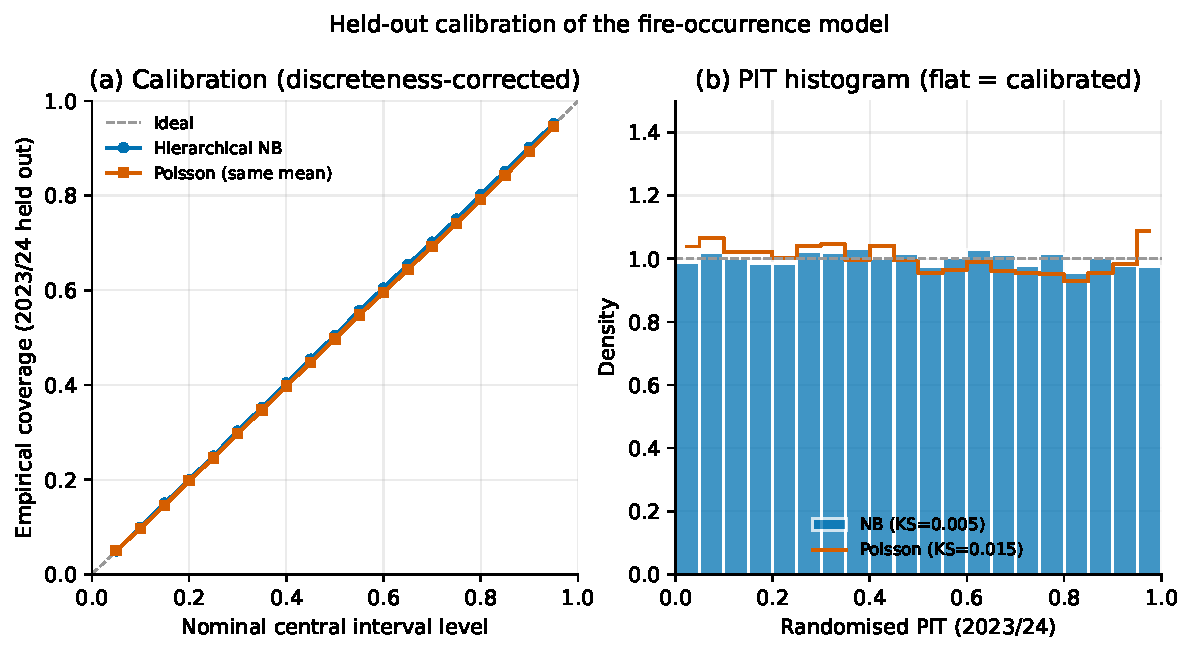
\includegraphics[width=0.8\linewidth]{figures/occ_calibration.pdf}
  \caption{Held-out calibration of the occurrence model (FY 2023/24): coverage
  of central posterior-predictive intervals (left) and randomised-PIT histogram
  (right). The PIT is close to Uniform, indicating good discrete-count
  calibration.}
  \label{fig:occ-cal}
\end{figure}

\begin{figure}[htbp]
  \centering
  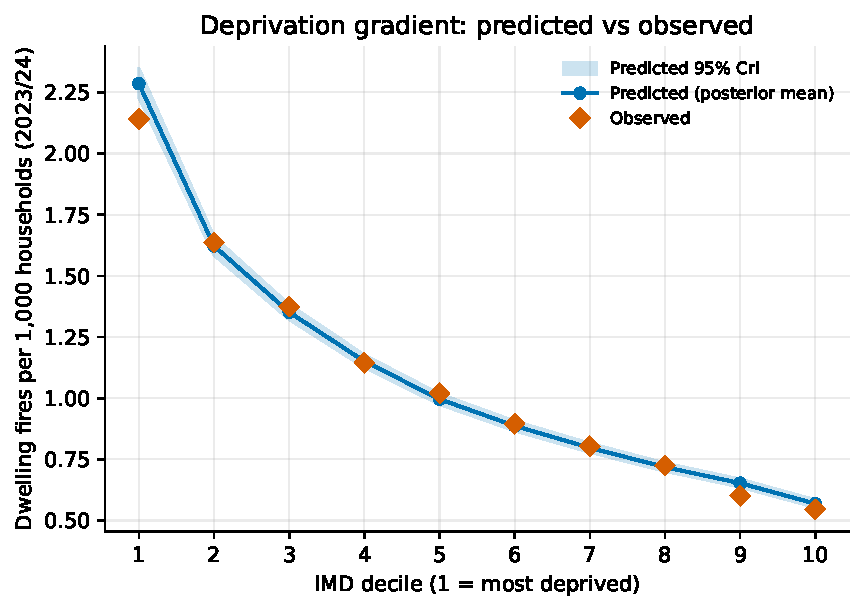
\includegraphics[width=0.55\linewidth]{figures/occ_decile_gradient.pdf}
  \caption{Dwelling-fire rate per 1{,}000 households by IMD decile, predicted
  vs observed. The monotone deprivation gradient is reproduced. Covariate rate
  ratios are in Table~\ref{tab:occ-forest}.}
  \label{fig:occ-decile}
\end{figure}

\paragraph{Robustness (full-data, ablation, spatial, subgroups).}
Three checks confirm the model. The exact full-data posterior above is
corroborated by an independent full-data ADVI refit, which
reproduces every rate ratio to within 0.022 and \emph{strengthens} the
overdispersion result --- the equal-mean Poisson undercovers badly (50\% interval
covers 0.401) while the negative binomial stays on target (0.503 / 0.901). An
ablation ladder (Table~\ref{tab:ablation}) shows deprivation is by far the largest
single gain, the EPC covariate adds essentially nothing at LSOA level, and a
Besag--York--Molli\'e (BYM2) spatial random effect removes the residual spatial
autocorrelation the service intercepts leave (Moran's $I$ falls $0.059\to-0.086$) for
only a small held-out gain --- real but modest, and this M5 specification is preferred
over the rejected quadratic-year M6. And calibration holds \emph{within} subgroups:
held-out PIT--KS stays near 0.01 across IMD quintiles, urban/rural strata and
\%-flats tertiles, with median 0.039 across the 43 service areas.

\begin{table}[htbp]
  \centering
  \caption{Occurrence ablation ladder (full-data variational fits, so M5 point
  estimates differ slightly from the exact posterior of
  Table~\ref{tab:occ-forest}), held-out
  2023/24. Deprivation dominates; the EPC covariate adds nothing at LSOA level; the
  intrinsic-conditional-autoregressive (ICAR)-based BYM2 spatial effect is real but
  modest; the preferred model is M5. Log-score is NB held-out log predictive density
  (higher is better).}
  \label{tab:ablation}
  \small
  \begin{tabular}{@{}lcccc@{}}
    \toprule
    Rung & Log-score & PIT--KS & cov50 & cov90 \\
    \midrule
    M0 intercept + trend        & $-1.1725$ & 0.0056 & 0.506 & 0.902 \\
    M1 + deprivation            & $-1.1155$ & 0.0047 & 0.504 & 0.900 \\
    M2 + building form (Census) & $-1.1024$ & 0.0044 & 0.504 & 0.902 \\
    M3 + EPC covariate          & $-1.1024$ & 0.0045 & 0.503 & 0.902 \\
    M4 + service random effect  & $-1.1000$ & 0.0039 & 0.502 & 0.901 \\
    \textbf{M5 + BYM2 spatial (preferred)} & $-1.0976$ & 0.0053 & 0.495 & 0.898 \\
    M6 + quadratic year (rejected) & $-1.0963$ & 0.0146 & 0.505 & 0.904 \\
    \bottomrule
  \end{tabular}
\end{table}

\subsection{Consequence severity}
\label{sec:results-casualty}

Two record-level outcomes are modelled from the 451{,}172 dwelling-fire records by
hierarchical Bayesian logistic regression, each with an FRS-level random intercept.
\emph{Serious spread} is fire leaving the room of origin (a direct proxy for
compartmentation failure); \emph{any-casualty} is the data-protected binary
casualty indicator (fatalities cannot be separated from non-fatal casualties at
record level). The models are fit by \emph{exact} NUTS on all 451{,}172 records
--- no subsampling --- trained on FY 2010/11--2022/23 ($n=400{,}250$) and
evaluated out-of-time on 2023/24--2024/25 ($n=50{,}922$), with every reported
fixed effect converged cleanly ($\hat{R} \le 1.02$, zero divergences). A
fiscal-year-stratified subsample fit ($n=29{,}999$) and an independent
maximum-likelihood (MLE) fit on the full records serve as cross-checks under the
two-track protocol of Section~\ref{sec:model}, reproducing the same effect signs
and comparable magnitudes. The current specification adds an
FRS-year \emph{response-time context} covariate --- the mean total call-to-arrival
delay per FRS and fiscal year from FIRE1001, joined exactly to every incident (0\% unmatched) and
standardised (1\,SD $\approx 1.23$ minutes about a 7.71-minute mean). Both models
are well calibrated out-of-time: expected calibration error (ECE) is 0.0096 for
spread and 0.0108 for casualty, and held-out area under the
receiver-operating-characteristic curve (AUC) is 0.752 and 0.685 respectively
(Figure~\ref{fig:cons-cal}); per-service interval coverage is discussed under
robustness below.

Response time itself carries only a weak, non-robust signal and must be read as an
\emph{ecological} exposure, not an incident-level measurement: it varies only at
FRS$\times$year resolution, so with the FRS random intercept absorbing between-area
differences it is identified largely from within-FRS year-to-year variation and is
partly entangled with the secular fiscal-year trend. On the subsample the casualty
odds ratio (OR) per $+1$\,SD is 0.851 (95\% CrI [0.777, 0.931]) and the spread OR
0.922 ([0.851, 0.993]); but on the full 451{,}172 records the spread effect
\emph{flips sign} (OR 1.052, [1.018, 1.084]) while casualty stays below one
(0.944, [0.915, 0.973]). We therefore report no directional response-time effect on spread, and read
the (still ecological, non-causal) casualty association only weakly; the covariate is
retained as a control, not a finding.

The headline effect is the alarm ladder (Table~\ref{tab:alarm}). For serious
spread the signal is clean and mechanistically sensible: relative to a working
alarm, a fire with \emph{no} alarm has 1.65 times the odds of spreading beyond the
room of origin (OR 1.653, 95\% CrI [1.610, 1.693]), and an alarm present that did
not raise the alarm carries the highest odds of all (OR 2.401). Detection cuts
spread. The casualty model, however, shows the no-alarm odds ratio falling
\emph{below} one (OR 0.786, [0.766, 0.804]). This sign flip is not an alarm being
harmful; it is the expected observational confound. A dwelling fire only produces a
casualty when someone is present and the fire is serious, and those same conditions
are what make an installed alarm sound --- so alarm operation is correlated with
exactly the occupancy and severity that raise casualty risk. Figure~\ref{fig:dag}
draws this backdoor path explicitly. The record-level data
cannot by itself identify the causal casualty-prevention effect; it identifies
adjusted associations. We report both outcomes precisely because the contrast ---
a clean detection$\to$spread signal alongside a confounded casualty association ---
is the motivating case for the latent-state layer of Section~\ref{sec:model},
whose job is to de-confound occupancy from detection. Reassuringly, the alarm
ladder is essentially unchanged by adding the response-time covariate (assessed on
the subsample track: the no-alarm spread OR moves 1.699$\to$1.701 and the no-alarm
casualty OR is unchanged) while calibration slightly improves, so the alarm
signal is robust to the new covariate. Other effects are large and interpretable:
chip/fat-pan fires multiply casualty odds by 3.25, lone pensioners by 2.21, and
night ignition by 1.83; purpose-built high-rise flats have the lowest spread odds
of any dwelling type (OR 0.378 vs houses), consistent with their compartmentation.

\begin{figure}[htbp]
  \centering
  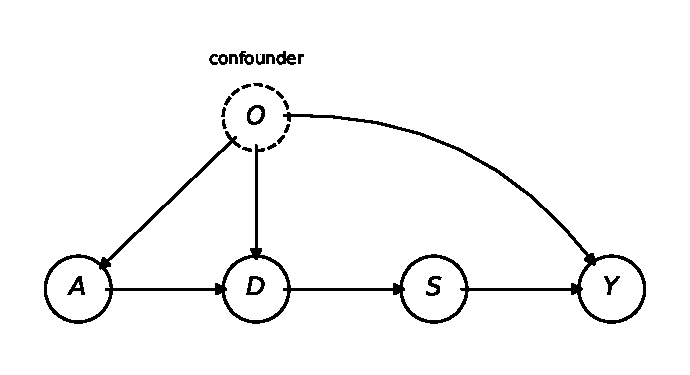
\includegraphics[width=0.55\linewidth]{figures/dag.pdf}
  \caption{Causal structure behind the alarm--casualty association. Occupancy $O$
  (dashed, the confounder) opens the backdoor path $A \leftarrow O \rightarrow Y$:
  occupied, well-maintained dwellings both carry a working alarm ($O\rightarrow A$)
  and contain someone who can be harmed ($O\rightarrow Y$), and present occupants
  themselves aid detection ($O\rightarrow D$), while the alarm reaches casualties
  only along the causal chain $A\rightarrow D\rightarrow S\rightarrow Y$ (alarm $A$,
  detection $D$, severity/spread $S$, casualty $Y$). An adjusted no-alarm casualty
  odds ratio below one is the expected signature of this structure --- alarm
  operation tracks the very occupancy that raises casualty risk --- rather than a
  protective effect of \emph{removing} alarms. The record-level data identify
  adjusted associations along this graph, whereas the intervention effect requires
  the do-operator treatment referenced in Section~\ref{sec:model}.}
  \label{fig:dag}
\end{figure}

\begin{table}[htbp]
  \centering
  \caption{Alarm ladder: odds ratios (95\% CrI) for each alarm state versus a
  working alarm (present and raised), adjusted for dwelling type, cause, ignition,
  occupancy, time, year, response time and FRS; exact NUTS posterior on all
  451{,}172 records. Detection lowers spread; the
  casualty column is confounded by occupancy (see text).}
  \label{tab:alarm}
  \small
  \begin{tabular}{@{}lcccc@{}}
    \toprule
    & \multicolumn{2}{c}{Serious spread} & \multicolumn{2}{c}{Any casualty} \\
    \cmidrule(lr){2-3}\cmidrule(lr){4-5}
    Alarm state vs.\ working & OR & 95\% CrI & OR & 95\% CrI \\
    \midrule
    Absent                       & 1.653 & [1.610, 1.693] & 0.786 & [0.766, 0.804] \\
    Present, did not operate      & 1.116 & [1.083, 1.148] & 0.789 & [0.769, 0.810] \\
    Present, did not raise alarm  & 2.401 & [2.329, 2.474] & 1.196 & [1.162, 1.230] \\
    \bottomrule
  \end{tabular}
\end{table}

\begin{figure}[htbp]
  \centering
  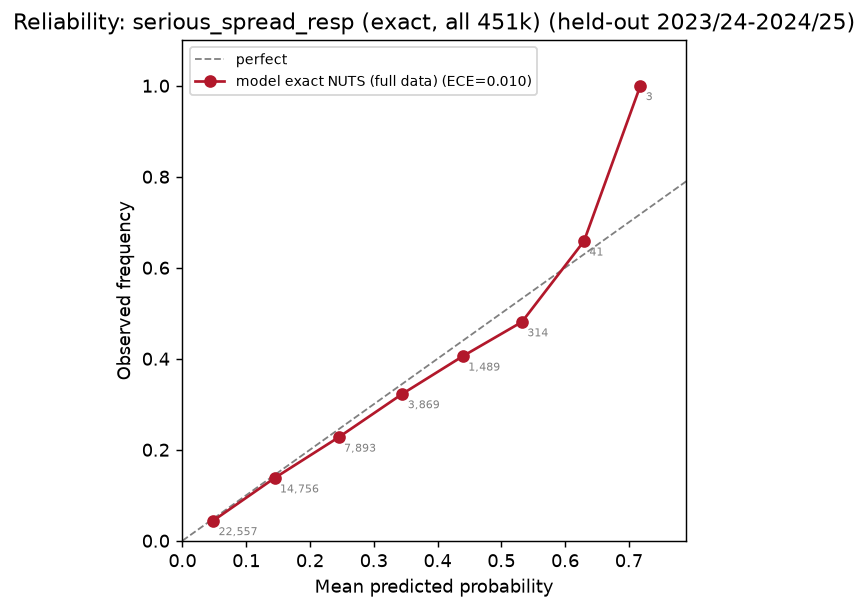
\includegraphics[width=0.7\linewidth]{figures/cons_reliability_spread.png}
  \caption{Out-of-time reliability curve for the serious-spread model
  (exact full-data NUTS, response-time specification, FY 2023/24--2024/25),
  ECE 0.0096. Predicted probabilities track observed frequencies across bins.}
  \label{fig:cons-cal}
\end{figure}

\paragraph{Robustness (proper scores, full data, subgroups).}
Because the area under the ROC curve alone is a weak test for rare outcomes, we also
report strictly proper scores (Table~\ref{tab:proper}): the hierarchical model beats an
intercept-only baseline decisively on the Brier score, mean log score and
precision--recall AUC (PR-AUC), matches a plain logistic while adding calibrated
uncertainty, and sits well above the PR-AUC base-rate floors ($\approx0.15$ / $0.13$).
The exact full-data posterior agrees with the subsample track, full-data ADVI and
full-data MLE on every headline effect (no-alarm casualty OR $0.758\to0.786$,
spread $1.70\to1.65$), and its $\sim$4$\times$ tighter intervals resolve two
subsample artefacts: the deliberate-cause casualty OR collapses from a wide,
nominally significant 3.04 [1.05, 10.6] to a clean null (1.12, [0.92, 1.38]), and
the response-time spread coefficient settles at the sign discussed above. One
honest caveat surfaces at scale: the full-data fits undercover per-FRS held-out
counts (0.81 for spread and 0.65 for casualty under exact NUTS, versus 1.00/0.93
on the subsample), and since the \emph{exact} sampler undercovers too this is a
real FRS-overdispersion gap (out-of-time drift and within-service heterogeneity a
single intercept misses), not a variational artefact --- fixed effects are best
estimated from the full data, while per-service predictive intervals from the
tighter full-data posterior should be read as anti-conservative and a
random-slope extension is future work. Calibration broadly holds \emph{within} alarm,
dwelling-type and time-of-day subgroups (most subgroup expected calibration errors of
the same $0.01$--$0.02$ order as the marginal figure, with larger wobbles at
small-$n$ cells such as bungalows, ECE $0.09$ at $n{=}189$).

\begin{table}[htbp]
  \centering
  \caption{Held-out proper scores for the consequence models versus an intercept-only
  baseline (subsample held-out, $n=3{,}386$). Lower Brier and log score are better;
  higher PR-AUC and ROC-AUC are better. The hierarchical model ranks rare events well
  above the base-rate floor.}
  \label{tab:proper}
  \small
  \begin{tabular}{@{}llcccc@{}}
    \toprule
    Outcome & Model & Brier & Log score & PR-AUC & ROC-AUC \\
    \midrule
    Casualty       & Hierarchical    & 0.1205 & 0.3984 & 0.245 & 0.659 \\
    Casualty       & Intercept-only  & 0.1250 & 0.4166 & 0.146 & 0.500 \\
    Serious spread & Hierarchical    & 0.1041 & 0.3446 & 0.318 & 0.757 \\
    Serious spread & Intercept-only  & 0.1160 & 0.3939 & 0.134 & 0.500 \\
    \bottomrule
  \end{tabular}
\end{table}

\subsection{Interaction structure: who gains most from an alarm}
\label{sec:results-interactions}

Does the alarm benefit differ by occupancy, and the night penalty by dwelling type?
We add two interactions to the consequence model --- alarm$\times$occupancy and
night$\times$dwelling-type --- and, because interaction cells are noisy, hold them to
a strict discipline: a joint likelihood-ratio (LR) test of each interaction block on
the full data, Benjamini--Hochberg false-discovery-rate (BH-FDR) control across cells,
and a dual gate that calls a cell robust only if it clears \emph{both} the Bayesian
95\% credible interval and the full-data maximum-likelihood interval with the same
sign. Of 68 tested cells, the robust ones are 8 (spread) and 5 (casualty) in
alarm$\times$occupancy and 2 (casualty) in night$\times$dwelling.

The spread channel --- the cleaner, less-confounded detection signal --- shows a
genuine \emph{occupancy gradient} in the value of a working alarm
(Figure~\ref{fig:int-ame}). The no-alarm-versus-working spread odds ratio runs from
about 3.30 [3.04, 3.57] for a lone person over pensionable age --- roughly double the
pooled 1.65 --- down to indistinguishable-from-none for families with children (who
have waking occupants to detect a fire). Lone pensioners, lone under-pensioners and
older couples all sit robustly above the pooled penalty (the cell probabilities are
reported as adjusted average marginal effects, AME). By contrast the night effect on
spread is a \emph{whole-stock} phenomenon: none of the seven dwelling deviations from
the house reference clears both gates, so no building form --- HMOs and converted
flats included --- is disproportionately worse at night once the shared night penalty
is removed. The interaction terms do not degrade calibration (held-out ECE
0.012--0.014). The targeting consequence is drawn out in
Section~\ref{sec:discussion}: the alarm benefit should be occupancy-modulated toward
lone pensioners, while night warrants no dwelling-specific multiplier.

\begin{figure}[htbp]
  \centering
  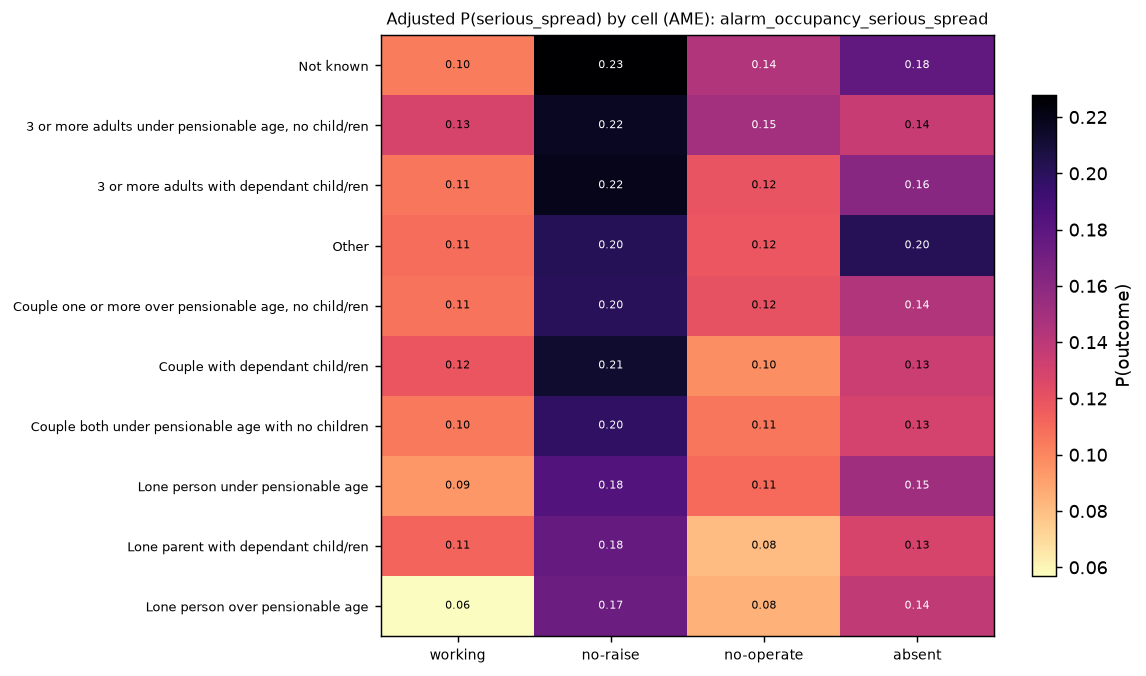
\includegraphics[width=0.82\linewidth]{figures/int_ame_alarm_occupancy.png}
  \caption{Adjusted probability of serious spread by occupancy type (rows) and alarm
  state (columns), from the alarm$\times$occupancy interaction. The no-alarm spread
  penalty is largest for lone pensioners, who gain the most containment from a working
  alarm.}
  \label{fig:int-ame}
\end{figure}

\subsection{Simulation and surrogate}
\label{sec:results-sim}

The evacuation-failure factor $P(E_f\mid S,I)$ comes from the archetype simulator
of Section~\ref{sec:surrogate}, run for 420{,}000 Monte Carlo ignitions (10{,}000
per archetype~$\times$~alarm~$\times$~time-of-day cell, fixed seed). Every parameter
is declared in a single assumptions registry with a provenance tag (calibrated to
data, consistent with PD~7974 and Society of Fire Protection Engineers (SFPE)
practice, grounded in the literature, or a transparent engineering estimate), so
the model is auditable rather than a black box. Table~\ref{tab:sim} gives the
headline night-time per-occupant evacuation-failure probabilities.

\begin{table}[htbp]
  \centering
  \caption{Per-occupant $P(\text{evacuation failure}\mid\text{ignition})$ at
  night, by archetype and alarm state (Monte Carlo, 95\% confidence intervals (CIs)
  in the full results).
  A working alarm roughly halves failure in most archetypes; the care home is the
  exception (see text).}
  \label{tab:sim}
  \small
  \begin{tabular}{@{}lccc@{}}
    \toprule
    Archetype & no alarm & alarm not working & working alarm \\
    \midrule
    detached house & 0.385 & 0.370 & 0.249 \\
    terraced house & 0.404 & 0.396 & 0.242 \\
    low-rise flat  & 0.141 & 0.132 & 0.049 \\
    high-rise flat & 0.071 & 0.068 & 0.012 \\
    HMO            & 0.364 & 0.355 & 0.262 \\
    care home      & 0.163 & 0.165 & 0.168 \\
    mixed use      & 0.181 & 0.176 & 0.070 \\
    \bottomrule
  \end{tabular}
\end{table}

The care home is the informative exception: its evacuation-failure rate barely
moves with alarm state (0.163 / 0.165 / 0.168 at night), because its bottleneck is
occupant \emph{mobility}, not \emph{detection} --- a 75\% mobility-impaired
population with long pre-movement times cannot exploit earlier warning under a
full-evacuation assumption. Detection helps where egress is fast (flats, houses);
it does not where egress is slow. This is exactly the kind of archetype-specific
mechanism the surrogate is meant to expose.

Against the observed dwelling-fire statistics the simulator is \emph{loosely}
calibrated --- we target orderings and magnitudes, not exact matches --- and the
orderings hold. Spread beyond the room of origin ranks working alarm $<$ not
working $<$ none (simulation 0.100 / 0.185 / 0.184 vs data 0.079 / 0.146 / 0.185)
and night $>$ day (0.176 vs 0.137, data 0.207 vs 0.117); the compartmentation
ordering is strong, with purpose-built flats almost never spreading beyond the
floor of origin. The one acknowledged discrepancy is that multi-storey
\emph{houses} over-predict spread beyond the floor (simulation $\approx$0.13 vs
data 0.05), because an open internal stair lets fire climb too readily; flats match
closely. The simulator also independently reproduces the same casualty confound
seen in the record data --- observed casualty rate is \emph{highest} with a working
alarm --- while its causal $P(E_f)$ correctly \emph{decreases} with a working
alarm, which is the interventional quantity the risk model needs.

The new building-type benchmarks (FIRE0301/0304) give the care-home and mixed-use
archetypes their first real calibration targets, and they validate the
institutional archetypes with no change to the simulator's parameters. The
care-home archetype's spread-beyond-room rate (0.079) matches the observed
`communal living' class almost exactly (0.082) and sits far below the commercial
classes (retail 0.203, food-and-drink 0.225), confirming its institutional
compartmentation is at the right level. On consequence, communal-living buildings
have the highest casualty-per-fire of the residential-type classes (0.110), and the
care-home archetype's per-occupant evacuation-failure rate (0.156) is the right
order of magnitude, overstating the observed per-occupant casualty rate by roughly
$1.4\times$; the building-level $P(\geq 1\ \text{occupant fails})$ of 0.528
overstates by construction far more ($\sim$$4.8\times$) --- both are the
no-staff-assist, stay-put- and sprinkler-free full-evacuation upper bound flagged
as a limitation, now quantified against data. Separately, the smoke-alarm operation rate
$P(\text{operated}\mid\text{present}) = 0.743$ (FIRE0703) and working-alarm
ownership 0.924 (FIRE0701) confirm the \emph{structure} of the three-way alarm
split --- both a large ``working'' and a large ``present-but-failed'' population ---
but they are timing-free aggregate counts, so no detection parameter was changed.

Finally, three logistic-regression surrogates map archetype features (storeys,
occupants, compartmentation, impaired fraction, alarm state, night) to the three
consequence probabilities, recovering the Monte Carlo cell probabilities with
$R^2 = 0.861$ (spread beyond room), $0.969$ (spread beyond floor) and $0.936$
(evacuation failure), all with interpretable coefficient signs and bootstrap
prediction intervals. This surrogate is the closed-form $\mathbb{E}[C\mid I]$
engine that plugs into Equation~\eqref{eq:consequence}
(Figure~\ref{fig:sim-fail}).

\begin{figure}[htbp]
  \centering
  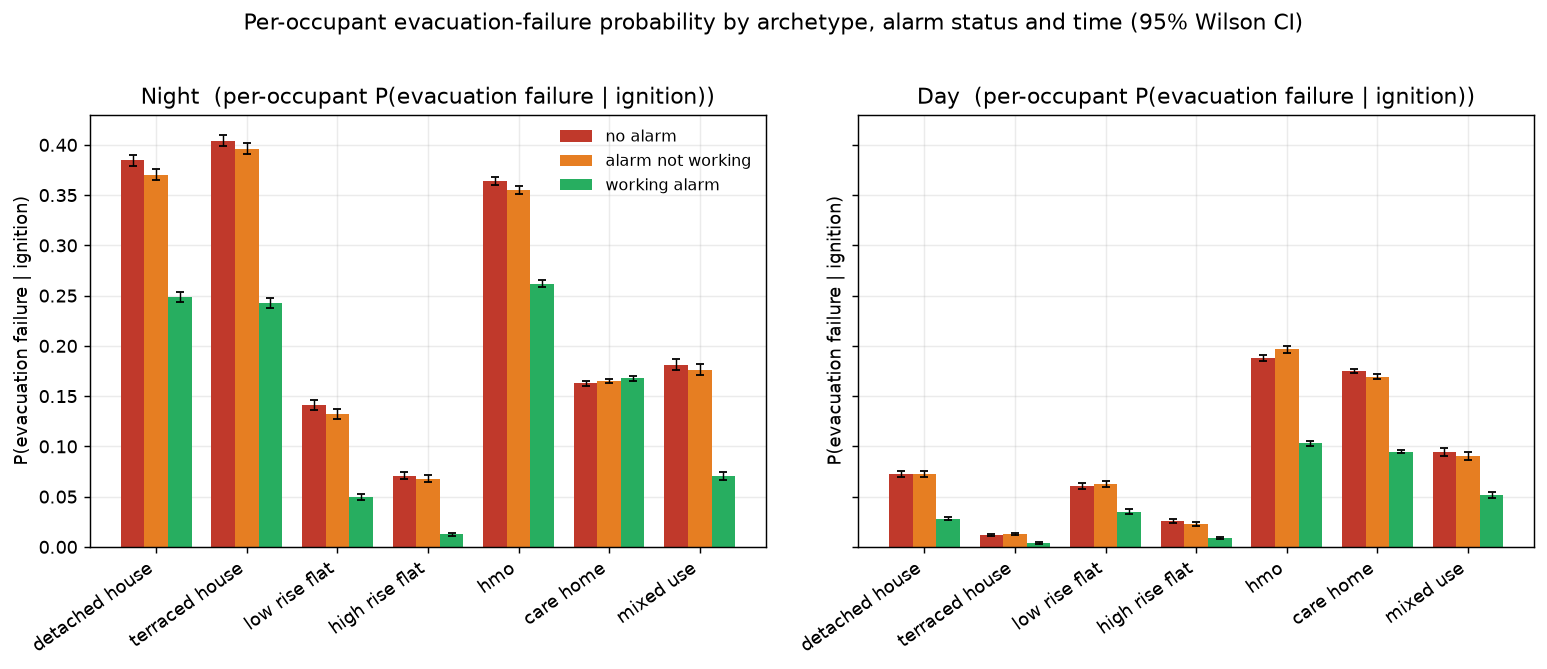
\includegraphics[width=0.82\linewidth]{figures/sim_failure_by_archetype.png}
  \caption{Per-occupant probability of evacuation failure by archetype, alarm
  state and time of day, with 95\% Monte Carlo error bars. A working alarm lowers
  failure in every archetype except the care home, whose bottleneck is mobility,
  not detection.}
  \label{fig:sim-fail}
\end{figure}

\subsection{Synthesis: a worked risk decomposition}
\label{sec:results-synthesis}

The three components combine into the posterior risk of
Equation~\eqref{eq:risk}, carrying uncertainty through each factor. Consider an
illustrative high-rise flat in a most-deprived-decile LSOA at night with no
working alarm. The occurrence model places the annual ignition probability near
the top of the deprivation gradient, $P(I)\approx 2.1\times10^{-3}$ per
household-year (Figure~\ref{fig:occ-decile}); the surrogate gives, for the
high-rise-flat archetype with no alarm at night, $P(S\mid I)\approx0.24$ and
$P(E_f\mid S,I)\approx0.071$. Composing these,
\begin{equation}
  R_b \;=\; \underbrace{P(I)}_{\approx 2.1\times10^{-3}}\;\cdot\;
  \underbrace{P(S\mid I)}_{\approx 0.24}\;\cdot\;
  \underbrace{P(E_f\mid S,I)}_{\approx 0.071}\;\cdot\;
  \mathbb{E}[L\mid\cdot]
  \;\approx\; 3.6\times10^{-5}\cdot\mathbb{E}[L\mid\cdot]\ \text{per hh-year},
  \label{eq:worked}
\end{equation}
before the loss term. Fitting a working alarm collapses the middle factor toward
$P(S\mid I)\approx0.09$ and the egress factor to $P(E_f\mid S,I)\approx0.012$, an
order-of-magnitude reduction in the evacuation-failure contribution --- the
quantitative expression of the intervention. To collapse these alarm-conditional
outputs into a single population-average consequence for a stock of mixed alarm
reliability, the surrogate's working and not-working predictions are combined using
the empirical smoke-alarm operation rate $P(\text{operated}\mid\text{present})=0.743$
(FIRE0703; Section~\ref{sec:results-sim}) as the population weight --- supplied to
the risk model rather than baked into the simulator. Crucially each factor carries a
credible interval (the occurrence posterior, the consequence-model CrIs of
Table~\ref{tab:alarm}, and the surrogate's bootstrap prediction intervals), so the
product in Equation~\eqref{eq:worked} is a \emph{distribution} over $R_b$, not a
point score, and the width of that distribution is itself the missing-evidence
signal that drives inspection prioritisation (Section~\ref{sec:model-inspection}).
These figures are illustrative of the composition rather than a calibrated
building-level prediction; building-level validation remains at the aggregate level
(Section~\ref{sec:discussion}).

\subsection{Decision layer: value of targeted prevention}
\label{sec:results-decision}

The framework exists to support decisions, so we close the analysis with a worked
value-of-inspection demonstration (contribution~4): given a \emph{fixed} prevention
budget, how much better can a fire and rescue service target it using the calibrated
posteriors than with untargeted or deprivation-only rules? This is emphatically
\emph{not} an argument against statutory fire risk assessment --- PAS~79
\citep{pas79_1_2020}, the Building Safety Act and the post-Grenfell regime are valued
safety improvements. The decision layer is a quantitative prioritisation layer that
\emph{backs} that regime with data: which homes, in which order, for a limited
budget. The policy evaluated is a real intervention --- FRS home fire-safety
(``Safe and Well'') visits that install or check a working smoke alarm --- at a fixed
budget of 100{,}000 visits across England. Four ranking rules are evaluated against
the same world (Table~\ref{tab:decision}): random, IMD-decile (current common
practice), posterior fire rate, and a full expected-benefit rule that is
uncertainty-aware and consequence-valued (rate~$\times$~$P(\text{no working
alarm})$~$\times$~$P(\text{casualty}\mid\text{fire})$~$\times$~relative risk
reduction (RRR)).

Economic values are the Home Office \emph{Economic and Social Cost of Fire}
\citep{homeoffice2023costfire}: averting one casualty-fire is worth \pounds66{,}113
(national-average severity, dominated by the rare fatality) and a working alarm
averts an assumed 20\% of a fire's \pounds14{,}009 property damage; benefits accrue
over a 10-year alarm life discounted at 3.5\% (present value (PV) multiplier 8.61)
against a \pounds55 visit cost. The alarm's causal effect is taken from the
\emph{interventional} surrogate rather than the confounded observational casualty
odds ratio (which is below one), and is cross-checked against the observational
spread signal; every causal assumption is tabled with a sensitivity sweep.

Targeting multiplies the return roughly ninefold: expected-benefit targeting returns
\pounds0.71 per \pounds1 spent versus \pounds0.078 for random allocation, and averts
3.1 casualty-fires per year against 0.34 (Table~\ref{tab:decision}). The calibrated
occurrence model also beats the
deprivation proxy by about $2.5\times$ (3.0 vs 1.2 casualty-fires averted for
posterior-risk vs IMD-decile targeting): deprivation is a genuinely strong single
proxy --- it co-varies with fire rate, the alarm gap and vulnerability at once, which
is why services use it and we treat it respectfully --- but within the deprived
deciles the calibrated model pinpoints the specific high-rate LSOAs that
random-within-decile misses. The consequence and uncertainty-aware signals add a
further modest gain (0.705 vs 0.673); they are collinear with the fire rate here, so
once the rate is modelled well they add little, and they would matter more where
consequence decouples from occurrence. The absolute return sits below
\pounds1/\pounds1 by construction: we value \emph{only} the alarm's consequence
channel and exclude the visit's fire-prevention advice and health co-benefits, so
every figure is a deliberate lower bound. The contribution is the targeting
multiplier and the uncertainty-aware decision rule, not a claim that alarm
installation pays for itself on casualties alone; a sensitivity sweep shows the break-even frontier crossing the plausible
parameter region --- reached around a \pounds30 visit cost at the base effect
size, and requiring correspondingly larger interventional effects at higher
costs (Figure~\ref{fig:decision-sens}).

\begin{table}[htbp]
  \centering
  \caption{Value of targeting a fixed 100{,}000-visit smoke-alarm budget under four
  ranking rules, evaluated against the same England-wide world. Present value over a
  10-year alarm life at 3.5\%, casualty plus property, with 90\% credible intervals
  propagated from the occurrence posterior and surrogate bootstrap.}
  \label{tab:decision}
  \small
  \begin{tabular}{@{}lrcc@{}}
    \toprule
    Policy & LSOAs & Casualty-fires averted/yr & \pounds saved per \pounds spent \\
    \midrule
    (a) Random               & 33{,}755 & 0.34 [0.33, 0.35] & 0.078 [0.076, 0.080] \\
    (b) IMD decile           & 145      & 1.19 [1.15, 1.24] & 0.274 [0.267, 0.282] \\
    (c) Posterior risk       & 127      & 3.00 [2.87, 3.14] & 0.673 [0.649, 0.697] \\
    (d) Expected benefit     & 127      & 3.13 [2.99, 3.29] & 0.705 [0.678, 0.731] \\
    \bottomrule
  \end{tabular}
\end{table}


\paragraph{Formal allocation, value of inspection, and budget size.}
The allocation is the constrained maximisation of expected averted loss of
Equation~\eqref{eq:knapsack}; because every dwelling in an LSOA shares the same
marginal value, it is a continuous knapsack whose optimum is the greedy rule (rank by
marginal value, fill from the top), and policy (d) is its Bayes action --- ranking by
posterior-mean averted loss. Reframing the visit as an inspection that resolves alarm
ownership gives the EVI of Equation~\eqref{eq:evi}, which sharpens the picture: the
prior-optimal action is to visit in only 0.04\% of dwellings (expected benefit exceeds
the \pounds55 cost almost nowhere), yet a visit \emph{would} pay in the 29.0\% of
dwellings that turn out to lack a working alarm --- so the programme's whole value lies
in \emph{finding} those homes, which is what inspection does, with total EVI over
England $\approx\pounds22.7$m. EVI is also a genuinely different ranking from expected
risk (Spearman $\rho=0.79$, versus $0.985$ for expected-benefit-versus-risk): it zeroes
out the $\sim$71\% of areas where a visit can never pay, so uncertainty-reducing
targeting is distinct from risk targeting even though the two coincide on the top LSOAs
a 100{,}000-visit budget reaches.

The headline economic result is a break-even one, and it is about concentration, not
scale. Sweeping the budget (Table~\ref{tab:budget}), a small, tightly targeted
10{,}000-visit programme clears break-even on the smoke-alarm channel alone
(\pounds1.12 per \pounds1) even on our conservative casualty-plus-property valuation;
the advantage over IMD targeting then falls from $4.4\times$ at 10{,}000 visits to
$1.4\times$ at one million as a larger programme is pushed down into lower-risk stock.
A decision-curve analysis and the visit-cost$\times$effect-size sensitivity map
(Figure~\ref{fig:decision-sens}) place the break-even frontier inside the plausible
region: cheaper visits or the upper half of the effect-size range lift the channel
above \pounds1/\pounds1.

\begin{table}[htbp]
  \centering
  \caption{Return per pound (present value, casualty plus property) by programme size
  and policy. A small, tightly targeted programme clears break-even (\pounds1.12);
  the targeting advantage over IMD decays with scale (classic diminishing returns).}
  \label{tab:budget}
  \small
  \begin{tabular}{@{}rcccc@{}}
    \toprule
    Visits & Random & IMD decile & Posterior risk & Expected benefit \\
    \midrule
    10{,}000    & 0.078 & 0.252 & 1.112 & \textbf{1.119} \\
    50{,}000    & 0.078 & 0.255 & 0.800 & 0.821 \\
    100{,}000   & 0.078 & 0.256 & 0.673 & 0.704 \\
    250{,}000   & 0.078 & 0.261 & 0.545 & 0.563 \\
    500{,}000   & 0.078 & 0.260 & 0.449 & 0.464 \\
    1{,}000{,}000 & 0.078 & 0.267 & 0.362 & 0.374 \\
    \bottomrule
  \end{tabular}
\end{table}

\begin{figure}[htbp]
  \centering
  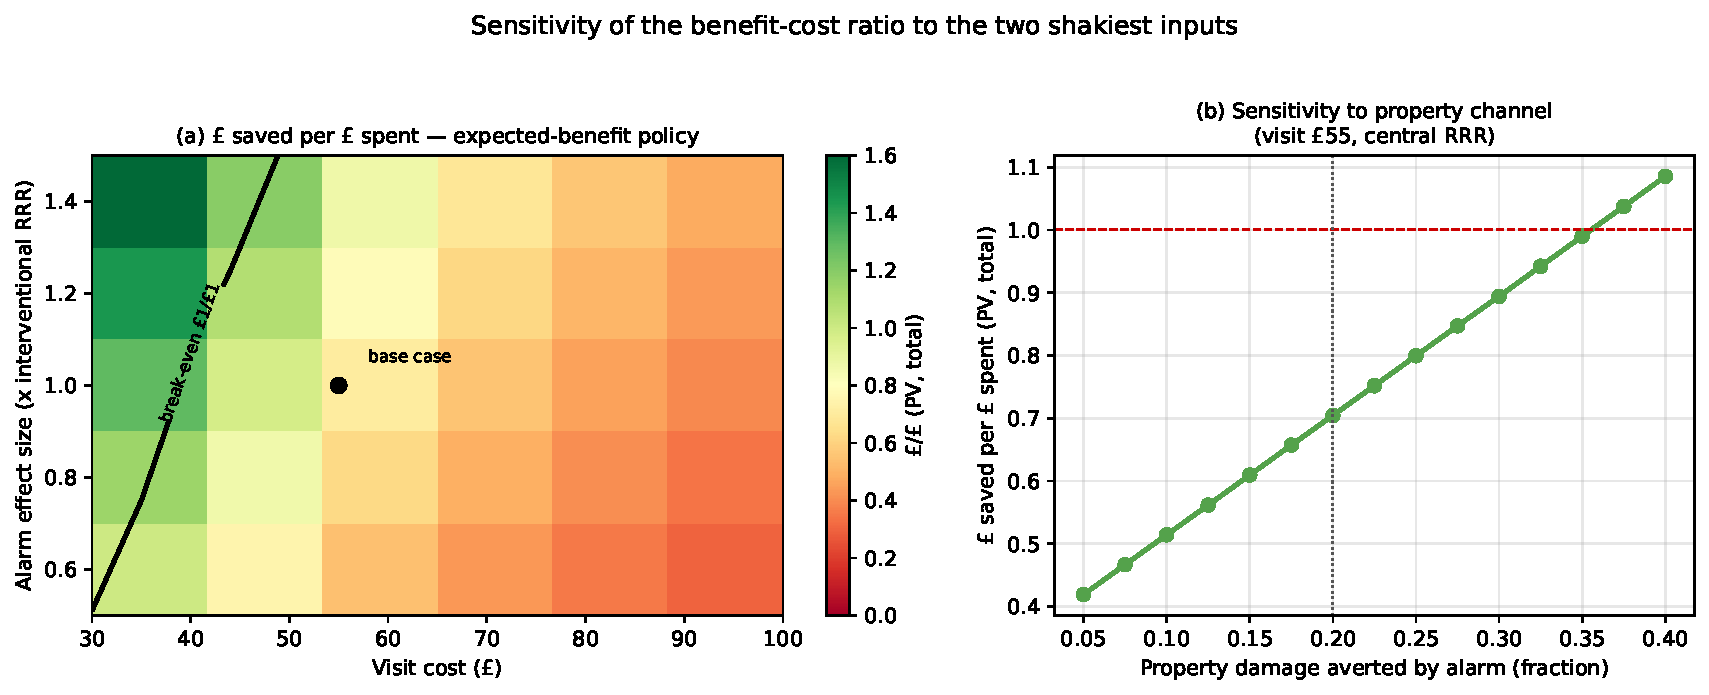
\includegraphics[width=0.78\linewidth]{figures/decision_sensitivity.pdf}
  \caption{Return per pound over visit cost (\pounds30--\pounds100) and alarm
  effect size (0.5--1.5$\times$ the interventional RRR), with the break-even contour
  and base-case marker. The frontier crosses the plausible region.}
  \label{fig:decision-sens}
\end{figure}

\paragraph{What finer geography buys: sub-LSOA concentration in London.}
The decision results above inherit the framework's granularity ceiling: the
national incident data resolve only to LSOA. London is the one fire service that
publishes incident records at finer resolution --- dwellings on a 50\,m grid ---
and a pilot on those records (90{,}318 dwelling fires, 2009--2024, with
EPC-derived dwellings per cell as exposure) shows how much that ceiling costs.
Within an average London LSOA, the top 10\% of inhabited 50\,m cells hold
\textbf{83\%} of the LSOA's dwelling fires, against 59\% expected from dwelling
density and small-count sampling noise alone (a dwelling-density multinomial
null; the honest signal is the 24-point excess). Priced with the same economics
as the policy comparison above, and evaluated \emph{out-of-sample} (cells
ranked on 2009--2020 by empirical-Bayes shrunk rates, every selected dwelling
scored at its realised 2021--2024 rate), cell-level targeting reaches dwellings
with \textbf{5.7$\times$} the fire rate of LSOA-level targeting at a
10{,}000-visit London budget --- lifting the smoke-alarm channel from
\pounds0.33 to \pounds1.88 saved per \pounds1 spent, i.e.\ above break-even
where LSOA targeting is not close (4.2--5.0$\times$ at larger budgets; a
perfect-foresight oracle reaches 11$\times$, the gap measuring how much apparent
concentration is noise). Both caveats push the estimate to be conservative: the
50\,m rounding coarsens true building-level concentration, and the $\sim$14\% of
fires falling outside EPC-covered cells are dropped from observed and null
alike (Figure~\ref{fig:london-targeting}). The implication is not that the
national model is wrong --- its calibration holds --- but that its geography
leaves roughly a sixfold value multiplier on the table, which is precisely the
case for record-level access to fine incident geography
(Section~\ref{sec:discussion}).

\begin{figure}[htbp]
  \centering
  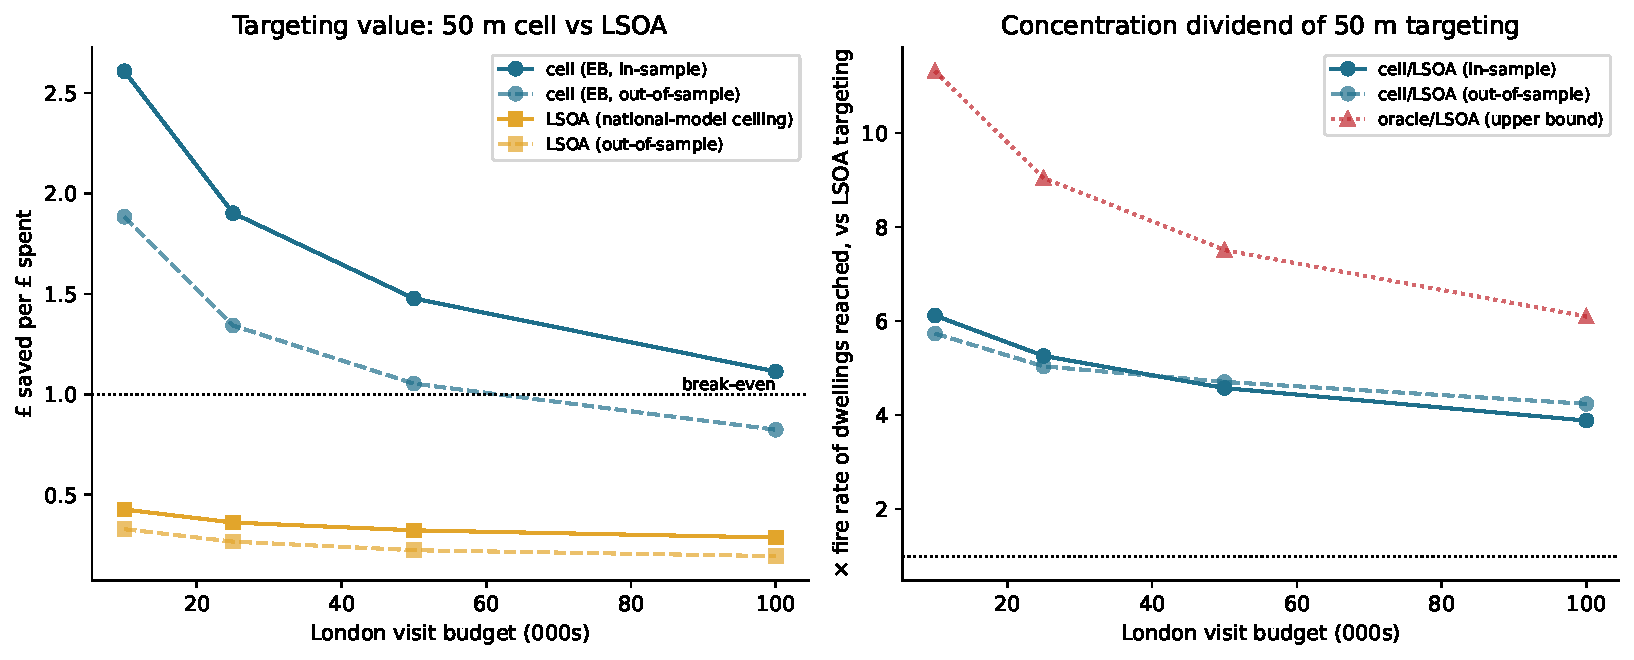
\includegraphics[width=0.85\linewidth]{figures/london_targeting.pdf}
  \caption{London pilot: out-of-sample value of sub-LSOA targeting. Cells ranked
  on 2009--2020 empirical-Bayes rates and scored on realised 2021--2024 rates;
  cell-level targeting reaches dwellings with 4.2--5.7$\times$ the fire rate of
  LSOA-level targeting across budgets, crossing break-even on the smoke-alarm
  channel alone at small budgets.}
  \label{fig:london-targeting}
\end{figure}

\subsection{Real-building stress test: Grenfell as a model-boundary case}
\label{sec:results-casestudy}

To probe how far the generic archetypes deviate from a real, exhaustively documented
building, we ground the high-rise-flat archetype against Grenfell Tower (14 June
2017), using only public evidence from the Grenfell Tower Inquiry Phase~1 report
\citep{grenfell2019phase1}. The 72 people who died are the reason this work exists;
the case study is framed in that spirit, and its purpose is to state plainly what a
population-scale interior model can and cannot represent. We rebuild the tower to its
real scale (24 storeys, six flats per floor, 120 residential flats, a single central
stair, 297 occupants present) with the same simulation engine and no change to any
parameter, and walk a one-variable-at-a-time path from the published archetype to the
real building (Table~\ref{tab:casestudy}).

The path isolates a clear finding: \emph{geometry barely matters; regime assumptions
dominate}. Placing the fire in the occupied flat --- the correct picture for the
exposed household under a stay-put design --- raises per-occupant evacuation failure
from 0.072 to 0.252 with no change in geometry. Replacing the generic 12-storey shape
with Grenfell's real 24-storey geometry then moves it only a further 2\% (0.252 to
0.258): doubling the storeys and adding flats per floor is nearly irrelevant to
whether the origin household escapes, because the single-stair topology the archetype
\emph{already} encodes is the safety-critical feature, and its compartmentation score
(1.356) essentially matches the real graph's (1.345). The catastrophe is a regime
change, not a geometry effect: losing compartmentation and forcing simultaneous full
evacuation takes per-occupant failure to 0.987 and expected fatalities from about 0.5
(one household) to about 293 (the whole building). The parameters that differ most
between archetype and reality --- the number of occupants in the evacuation problem
(2, the origin household under an intact stay-put design, vs 297, the whole building
once stay-put is revoked; per-flat occupancy is nearly identical at $\approx$2--2.5)
and storeys (12 vs 24) --- are \emph{not} the parameters that move the risk; whether compartmentation holds and
whether the building stays under stay-put are. The generic archetype is therefore a
sound geometric proxy whose one material simplification, shared by every archetype,
is that it presumes the design strategy holds.

Two honest boundaries follow. First, even in the breached case a working common alarm
with early simultaneous evacuation cuts expected fatalities from about 293 to about 4
--- the interior consequence of the post-Grenfell shift toward evacuation-alert
systems, which the model reproduces. Second, and decisively, \emph{our interior graph
has no external facade}. The mechanism that actually destroyed Grenfell --- flames
running up aluminium composite material (ACM) rainscreen cladding with polyethylene
cores and re-entering flats through failed windows on many floors at once --- lies
entirely outside a room--corridor--stair model, which is why the breached no-alarm
case predicts about 293 of 297 failing when 72 in fact died: it is a worst-case
envelope (no time-phased escape, a hard tenability cutoff), not a reconstruction. That
blind spot is not a defect to patch inside the model; it is the boundary between
population-scale interior risk ranking and the external-wall and safety-case regime
--- the combustible-cladding ban, Requirement~B4 external-fire-spread compliance
(which Grenfell failed), and the Building Safety Act's higher-risk-building regime ---
created precisely for the hazard our model cannot see. That division of labour is the
honest conclusion. Table~\ref{tab:grenfell-assumptions} makes the envelope explicit:
each simplification in the breached scenario removes a survival mechanism that
operated on the night, so every bias points the same way, and the two runs should be
read as brackets --- the event traversed from the intact regime toward the breached
one over roughly two hours, and the actual toll reflects who was still inside when
that transition completed.

Conditions (a) and (b) bracket the problem; a third condition (c) \emph{tests} it.
Feeding the model the documented Phase~1 fire timeline as an exogenous boundary
condition --- cladding involvement, an upward front of about one floor per minute,
lobby smoke-logging from $\approx$01:40, the single stair carrying significant smoke
from 02:00 --- and simulating only the egress and tenability response, with behaviour
calibrated \emph{solely} to the recorded departure anchor (``168 of 297 out by
01:50'', which the model reproduces at 176) and \emph{never} to the death toll, the
model predicts 37 expected fatalities (90\% Monte Carlo [28, 46]) against the actual
72 --- the right order of magnitude, under by about half (Table~\ref{tab:casestudy},
row (c)). This tests only the egress/tenability half of the model, since the hazard
field is imposed rather than derived. The miss is structured, not diffuse: a
five-parameter sensitivity sweep --- including the two per-floor stair-lethality
knobs that dominate the fatality count, each over its stated factor-of-two range ---
spans [12, 99] in expectation; constrained to departure curves consistent with the
observed anchor (155--185 out by 01:50), it spans [20, 73], so the true toll of 72
sits at the \emph{upper boundary} of the anchor-respecting envelope rather than
comfortably within it, and predicted fatalities rise with height as the documented
toll did. The central estimate reaches 72 only by pushing every dominant knob to its
lethal extreme; at plausible-central settings the tenability mechanics under-predict,
which localises the missing half to factors the model deliberately does not tune away:
occupant vulnerability held
at the archetype's 10\% impaired fraction (Grenfell's dead were disproportionately
disabled, elderly and children), coarse rescue and smoke modelling, and stay-put
maintained beyond survivable conditions --- the human and behavioural failures the
Inquiry identified. An honest, un-tuned under-prediction of this shape is more
informative than a fitted hit: the geometry and tenability mechanics are sound, and
the missing half lives in vulnerability and policy, not in the model's physics.

\begin{table}[htbp]
  \centering
  \caption{Breached-scenario assumptions vs the recorded event (Grenfell Tower
  Inquiry Phase 1). Every simplification removes a survival mechanism, so the
  scenario is a one-sided worst-case envelope: it predicts $\approx$293 of 297
  failing where 72 died. The intact-compartmentation run ($\approx$0.5 expected)
  is the opposite envelope, assuming the stay-put design works perfectly.}
  \label{tab:grenfell-assumptions}
  \small
  \begin{tabular}{p{0.30\linewidth}p{0.38\linewidth}p{0.22\linewidth}}
    \hline
    Model assumption (breached run) & What happened on the night & Bias on fatalities \\
    \hline
    Compartmentation lost building-wide at ignition &
    Progressive failure over $\sim$1--2\,h as the facade fire re-entered floor by
    floor & overstates \\
    Unaided self-evacuation only &
    Dozens rescued or assisted by firefighters & overstates \\
    Occupants move only when alerted, uniform compliance &
    168 of 297 had left by 01:50, many against stay-put advice, before its 02:47
    revocation; deaths concentrated among those who remained longest & overstates \\
    Stair degrades with the compartment loss &
    The single stair remained partially passable for hours despite smoke-logging &
    overstates \\
    Hard tenability cutoff, no refuge or relocation &
    Some occupants moved between flats and survived long after lobbies
    smoke-logged & overstates \\
    \hline
  \end{tabular}
\end{table}

\begin{table}[htbp]
  \centering
  \caption{Deviation path from the published archetype to real Grenfell geometry
  (rows a: night, no alarm). Per-occupant evacuation-failure probability and expected
  number of occupants failing to escape. Geometry moves the exposed-household risk by
  only 2\%; the regime change (lost compartmentation + full evacuation) moves it by
  two orders of magnitude. Row (c) is the as-unfolded hindcast under the imposed
  Phase~1 timeline (per-occupant fatality; predicted vs actual 72).}
  \label{tab:casestudy}
  \small
  \begin{tabular}{@{}lrcc@{}}
    \toprule
    Configuration & Occ. & $P(\text{fail}\mid\text{occ.})$ & $\mathbb{E}[\text{n fail}]$ \\
    \midrule
    Generic archetype (as published)          & 2   & 0.072 & 0.14 \\
    Generic geometry, fire in occupied flat    & 2   & 0.252 & 0.50 \\
    Grenfell geometry, intact (stay put)       & 2   & 0.258 & 0.52 \\
    Grenfell breached, full evacuation         & 296 & 0.987 & 292.5 \\
    \midrule
    (c) As-unfolded hindcast (imposed timeline) & $\sim$288 & 0.128 & 37 (actual 72) \\
    \bottomrule
  \end{tabular}
\end{table}

\subsection{Instantiating the inspection layer on real assessments}
\label{sec:results-latent}

The paper's proposed inspection-as-noisy-observation layer
(Section~\ref{sec:model}) is here fitted to real data for the first time: a corpus of
1{,}441 published fire risk assessments over 653 Camden council estates
\citep{camden_fra}, linked to London Fire Brigade primary-fire histories
\citep{lfb_incidents}. What is \emph{established} is the apparatus, not a positive
validity claim, and we state each part plainly.

\emph{The measurement model fits coherently.} A joint latent-factor model over the 653
estates recovers a single continuous latent deficit state $\theta$ whose measurement
model is the FRA indicators. They load coherently on it --- priority-A and priority-B
action counts, overall rating and the compartmentation, electrical and alarm flags all
move together (only the higher-risk-building-specific external-wall flag is near zero)
--- so $\theta$ is a well-defined ``assessed-deficiency'' state. Of the between-estate
log fire-rate variance attributed to $\theta$ plus the public deprivation covariate,
$\theta$ carries a median 94\%: the latent read off the inspection dominates the IMD
covariate in explaining where estate fire rates differ.

\emph{The posterior update works numerically.} For a worked single block (six flats,
most-deprived IMD decile, rating Moderate, nine actions, electrical and external-wall
flags), conditioning on its FRA observation through the measurement model turns a
prior expected fire rate of 0.027 fires/year (95\% CrI 0.016--0.048) into a posterior
of 0.025 (95\% CrI 0.017--0.036): the inspection both shifts and, more importantly,
\emph{narrows} the posterior (Figure~\ref{fig:latent}). This is
Equations~\eqref{eq:posterior-z}--\eqref{eq:posterior-R} made fully numeric for one
building --- the demonstration the framework promised.

\emph{The first empirical assessor-noise bounds exist.} Within-document ``raised in
previous report'' marks identify the compound of defect persistence and assessor
detection, not detection alone. Pooled recurrence fractions run 0.16--0.64 by
prior-action status; among blocks whose prior actions were left incomplete (high
persistence) the recurrence fraction 0.16 gives a \emph{lower bound} on detection
sensitivity $q$ of 0.16--0.32 across stated persistence assumptions
(Table~\ref{tab:bounds}). The compound is identified; sensitivity is only partially
identified --- point identification would need an actual re-inspection wave --- and we
claim no more.

A small true re-inspection pilot now exists: for eight blocks, an earlier assessment
of the same building (median gap eleven months) was recovered from public web
archives and compared item-by-item against the current one. Directly measured
persistence is high --- 84 of 121 wave-0 findings (69\%) match a finding in the new
assessment, ranging 61--83\% across matching thresholds --- yet \emph{none} of the
119 current-wave findings in these blocks carries the ``raised in previous report''
mark, against a corpus-wide marking rate of 22\%. The copy-forward marker is
therefore assessor- or document-dependent rather than systematic, so the recurrence
fractions above under-record true persistence and the sensitivity bounds are
conservative --- documentation noise of exactly the kind the measurement framework
models, now observed directly, in the first repeated-measurement FRA observations we
are aware of ($n=8$ pairs; a pilot and a pipeline rehearsal for the full second
wave, not a population estimate).

The validity analyses, reported honestly, are where the thesis meets the data. Do FRA
outputs track a block's long-run fire propensity? Regressing pre-assessment fires
(2009--23) on the later assessment, every estate-level rate ratio (RR) spans one. The
one block-level association excluding one --- the medium-priority (priority-B) action
count, RR 1.11 [1.03, 1.21] --- dies under estate-level aggregation (RR 1.00
[0.96, 1.04]), the unit robust to the fact that 54\% of blocks share an estate-centroid
coordinate, so we read it as a co-located-attribution artefact. The block-level compartmentation flag runs
\emph{negative} (more assessed deficiency, \emph{fewer} historical fires), while the
latent deficit state $\theta$ couples to fire rate as a null (RR 1.00 [0.69, 1.44],
$P(\beta_\theta>0)=0.50$) --- either no detectable coupling exists at this sample
size, or a true positive coupling is masked by the same
remediation-endogeneity mechanism the compartmentation flag exhibits --- assessors flag worse blocks, which then receive
remediation, cladding programmes and closer management that remove the very propensity
the flag marked --- \emph{not} evidence that deficiencies are protective. The cleanest
temporal test, whether prior incomplete actions predict fires in the following window,
is a low-power null (140 fires over $\approx$3.2-year windows; all intervals span one).

The interpretation is the paper's thesis meeting real evidence. A single FRA wave
cannot be read as a risk score --- it is confounded by remediation endogeneity and
limited by measurement noise --- which is precisely why the framework treats an
inspection as noisy evidence to be assimilated rather than as ground truth. What is
demonstrated is the apparatus (a coherent measurement model, a numeric
prior-to-posterior update, and the first bounds on assessor noise) on one borough's
council stock under a retrospective validity design; external validity is
unestablished, and de-confounding the structural coupling requires a second assessment
wave --- a Camden republication or a Freedom of Information (FOI) release of historical
FRAs --- the concrete data gap the programme's next stage targets.

\begin{table}[htbp]
  \centering
  \caption{Partial identification of assessor detection sensitivity $q$. The
  recurrence fraction among blocks with incomplete prior actions gives a conservative
  \emph{lower} bound on $q$ under an assumed defect-persistence $p$; the compound
  persistence$\times$detection is identified, $q$ alone is only bounded.}
  \label{tab:bounds}
  \small
  \begin{tabular}{@{}ccc@{}}
    \toprule
    Assumed persistence $p$ & $q$ lower bound & $q$ lower bound (95\% cons.) \\
    \midrule
    1.00 & 0.16 & 0.14 \\
    0.90 & 0.18 & 0.16 \\
    0.75 & 0.22 & 0.19 \\
    0.50 & 0.32 & 0.29 \\
    \bottomrule
  \end{tabular}
\end{table}

\begin{figure}[htbp]
  \centering
  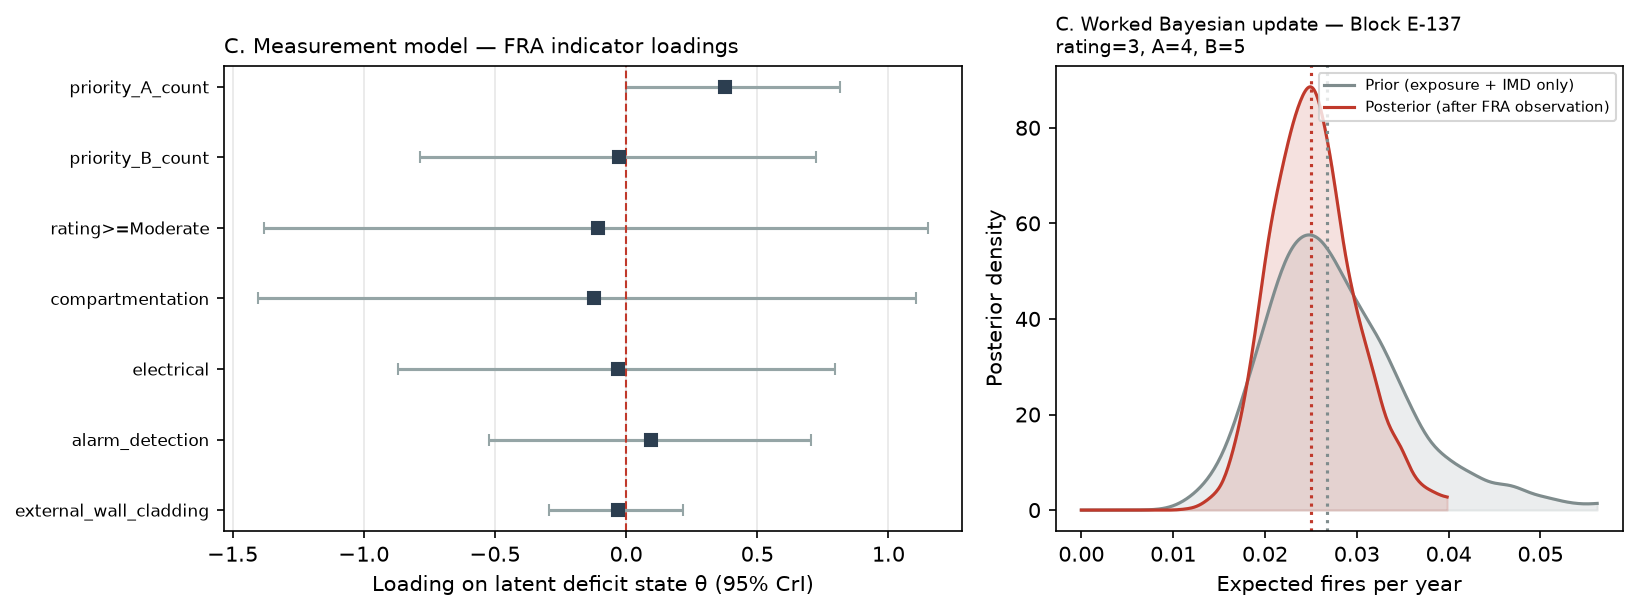
\includegraphics[width=0.9\linewidth]{figures/latent_worked_update.png}
  \caption{Worked single-block posterior update: conditioning on one estate's FRA
  observation shifts the expected fire-rate prior (95\% CrI 0.016--0.048 fires/year)
  to a tighter posterior (0.017--0.036). The inspection narrows the distribution ---
  the inspection-as-noisy-observation mechanism made numeric.}
  \label{fig:latent}
\end{figure}

\subsection{Ignition-source trends}
\label{sec:results-ignition}

Finally, a descriptive analysis of ignition sources over FY 2010/11--2024/25
(446{,}470 fires, Suffolk excluded from \emph{every} year to hold the 42-service
panel constant) fits a per-level generalised linear model (GLM) on fiscal year,
reporting each source's trend in its \emph{share} of dwelling fires
(Table~\ref{tab:ignition}, Figure~\ref{fig:ignition}). The clearest structural shift
is a broad, uniform decline in cooking-related ignition --- food as the ignited item
falls 10.8 percentage points, the single largest mover, alongside grills, hobs, ovens
and chip-pan fires --- consistent with safer appliance design. Against that backdrop
the fastest-rising identifiable source is the battery/electrical-apparatus family:
``battery charger'' fires rose $+425\%$ and ``apparatus --- batteries, generators''
$+86.8\%$, their combined share nearly tripling (1.28\% to 3.78\%, share odds ratio
1.059 per year).

The most useful finding, though, is a \emph{data-gap} one. The national taxonomy
cannot isolate the hazard the sector most fears: lithium-ion e-bike and e-scooter
fires have no dedicated category, and the only proxy (``batteries, generators'' plus
``battery charger'') nets device batteries with standby generators and predates the
e-mobility boom. London Fire Brigade's device-specific counts rose roughly thirtyfold
over 2017--2025 while the national proxy grew only about 72\% over fifteen years --- a
shape mismatch implying e-mobility fires are being absorbed into generic levels. We
flag this to MHCLG: a dedicated device-type sub-field is needed before the national
data can track this hazard. Separately, the rising ``Unspecified''/``Other'' buckets
($+2.6$ and $+2.0$ percentage points) are themselves a recording-drift flag --- a
growing ``don't know'' share erodes the precision of every other category, the battery
proxy included.

\begin{table}[htbp]
  \centering
  \caption{Biggest movers in ignition-source \emph{share} of dwelling fires,
  FY 2010/11--2024/25 (share odds ratio per year from a binomial GLM). The battery
  family rises fastest among identifiable sources; cooking-related sources fall
  broadly.}
  \label{tab:ignition}
  \small
  \begin{tabular}{@{}lccl@{}}
    \toprule
    Ignition source & $\Delta$ share (pp) & Share OR/yr & Trend \\
    \midrule
    Battery charger                      & $+0.44$  & 1.125 & rising ($+425\%$ count) \\
    Apparatus: batteries, generators     & $+2.06$  & 1.052 & rising ($+86.8\%$) \\
    Combined battery proxy               & $+2.50$  & 1.059 & rising \\
    Grill / toaster                      & $-3.02$  & 0.956 & falling \\
    Cooker incl.\ oven                   & $-0.72$  & 0.993 & falling \\
    Food (item ignited)                  & $-10.78$ & ---   & falling (largest mover) \\
    \bottomrule
  \end{tabular}
\end{table}

\begin{figure}[htbp]
  \centering
  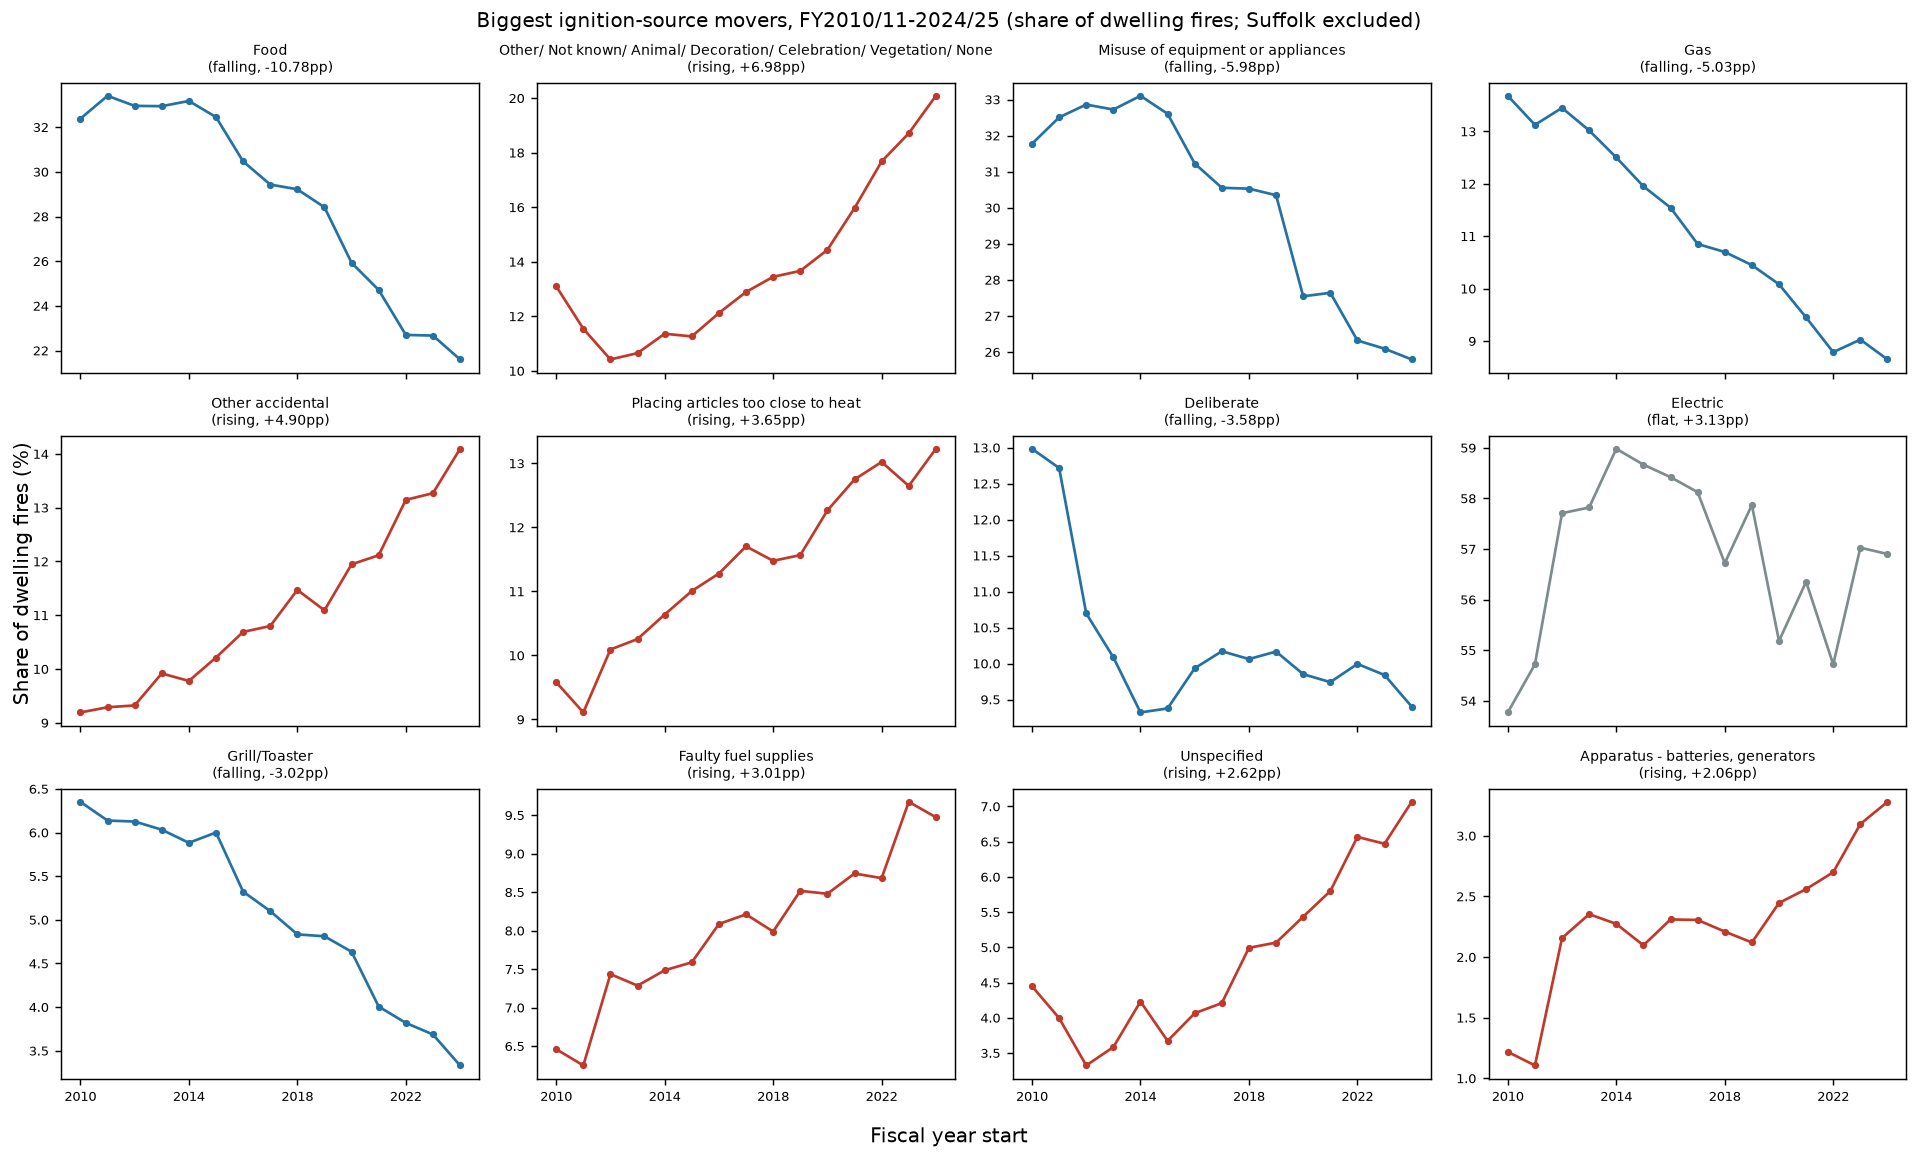
\includegraphics[width=0.82\linewidth]{figures/ign_small_multiples.png}
  \caption{Share trajectories of the twelve biggest-moving ignition sources, coloured
  by trend classification. Cooking sources decline broadly; the battery/apparatus
  family is the clearest riser after the generic ``Unspecified''/``Other'' buckets.}
  \label{fig:ignition}
\end{figure}
